\chapter{9. Iterator}
\section{Giới thiệu}
\subsection{Đặt vấn đề}
Trong khi phát triển các ứng dụng, chúng ta làm việc với nhiều loại tập hợp như: cấu trúc cây, mảng, tập hợp, bảng băm, ngăn xếp, hàng đợi, … Cách thức mà tập hợp này lưu trữ đối tượng của nó rất khác nhau, và nếu bạn muốn truy cập dữ liệu của những đối tượng này, bạn phải học những kỹ thuật khác nhau cho từng loại tập hợp. Khi đó, mẫu Iterator là một giải pháp tốt.\\
Chúng ta có thể sử dụng một interface được xác định phương thức cụ thể để truy cập tới từng phần tử của tập hợp. Sử dụng những phương thức này, chúng ta có thể truy xuất tới các phần tử trong tập hợp theo cùng cách dễ dàng nhất.

\begin{figure}[!htb]
    \centering
    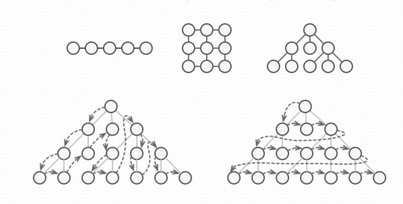
\includegraphics[width=\textwidth]{fig/Iterator/iterator_problem.png}
    \caption{Các loại tập hợp}
    \label{fig:iterator_problem}
\end{figure}

\subsection{Mục đích sử dụng}
\begin{itemize}
    \item Đảm bảo nguyên tắc Single responsibility principle (SRP) : chúng ta có thể tách phần cài đặt các phương thức của tập hợp và phần duyệt qua các phần tử (iterator) theo từng class riêng lẻ.
    \item Đảm bảo nguyên tắc Open/Closed Principle (OCP) : chúng ta có thể implement các loại collection mới và iterator mới, sau đó chuyển chúng vào code hiện có mà không vi phạm bất cứ nguyên tắc gì.
    \item Chúng ta có thể truy cập song song trên cùng một tập hợp vì mỗi đối tượng iterator có chứa trạng thái riêng của nó.
\end{itemize}

\section{Định nghĩa và mô hình cấu trúc}
\subsection{Định nghĩa}
Iterator Pattern là một trong những Pattern thuộc nhóm hành vi(Behavioral). Nó được sử dụng để “Cung cấp một cách thức truy cập tuần tự tới các phần tử của một đối tượng tổng hợp, mà không cần phải tạo dựng riêng các phương pháp truy cập cho đối tượng tổng hợp này.

\subsection{Mô hình cấu trúc}
\begin{figure}[!htb]
    \centering
    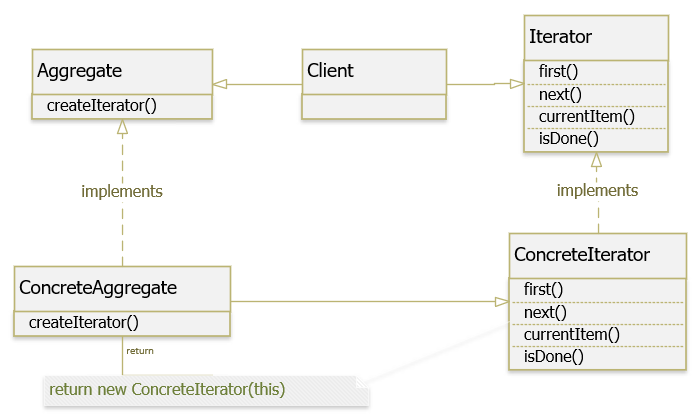
\includegraphics[width=\textwidth]{fig/Iterator/structure_iterator.png}
    \caption{Mô hình cấu trúc}
    \label{fig:structure_iterator}
\end{figure}

\begin{itemize}
    \item Aggregate : là một interface định nghĩa định nghĩa các phương thức để tạo Iterator object.
    \item ConcreteAggregate : cài đặt các phương thức của Aggregate, nó cài đặt interface tạo Iterator để trả về một thể hiện của ConcreteIterator thích hợp.
    \item Iterator : là một interface hay abstract class, định nghĩa các phương thức để truy cập và duyệt qua các phần tử.
    \item ConcreteIterator : cài đặt các phương thức của Iterator, giữ index khi duyệt qua các phần tử.
    \item Client : đối tượng sử dụng Iterator Pattern, nó yêu cầu một iterator từ một đối tượng collection để duyệt qua các phần tử mà nó giữ. Các phương thức của iterator được sử dụng để truy xuất các phần tử từ collection theo một trình tự thích hợp
\end{itemize}

\section{Cách cài đặt}
Cài đặt Iterator để duyệt qua các item trong một menu.\\
Link code cài đặt:
\url{https://github.com/nanhus/OOP-DesginPatten/tree/master/source/iterator}
\begin{figure}[!htb]
    \centering
    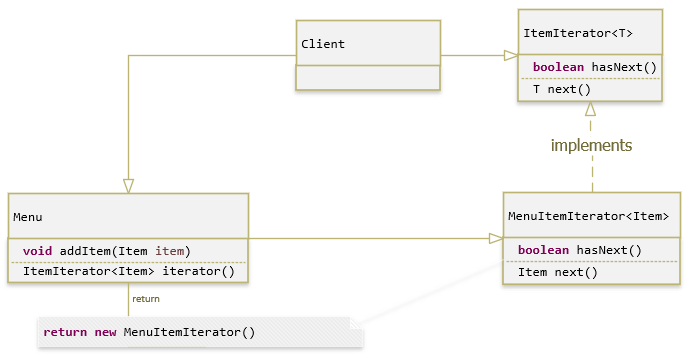
\includegraphics[width=\textwidth]{fig/Iterator/iterator_example.png}
    \caption{Mô hình cấu trúc}
    \label{fig:iterator_example}
\end{figure}
Dưới đây là code minh họa cài đặt:
\begin{figure}[!htb]
    \centering
    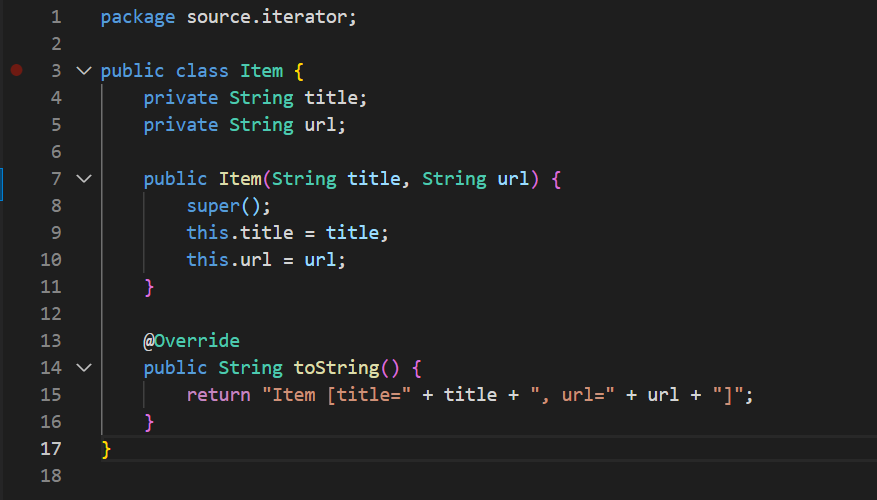
\includegraphics[width=\textwidth]{fig/Iterator/item_class.png}
    \caption{Item Class}
    \label{fig:item_class}
\end{figure}
\begin{figure}[!htb]
    \centering
    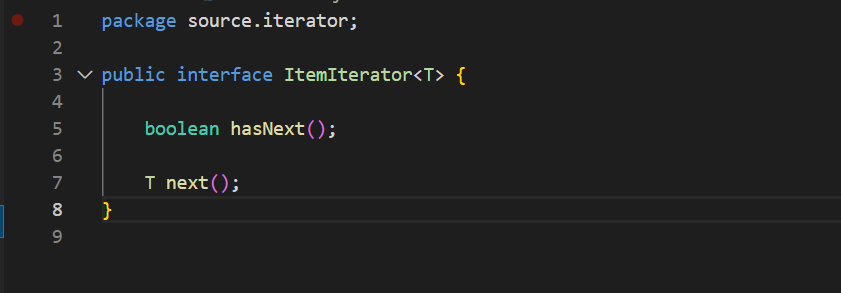
\includegraphics[width=\textwidth]{fig/Iterator/item_iterator_interface.png}
    \caption{Item Iterator Interface}
    \label{fig:item_iterator_interface}
\end{figure}
\begin{figure}[!htb]
    \centering
    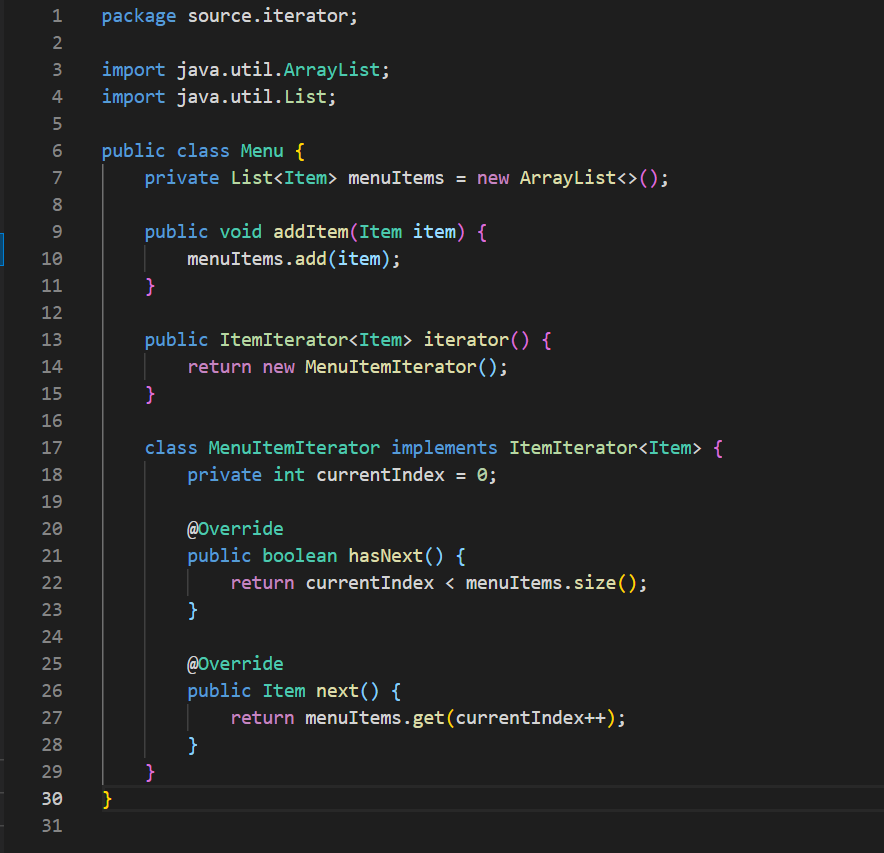
\includegraphics[width=\textwidth]{fig/Iterator/menu_class.png}
    \caption{Menu Class}
    \label{fig:menu_class}
\end{figure}
\begin{figure}[!htb]
    \centering
    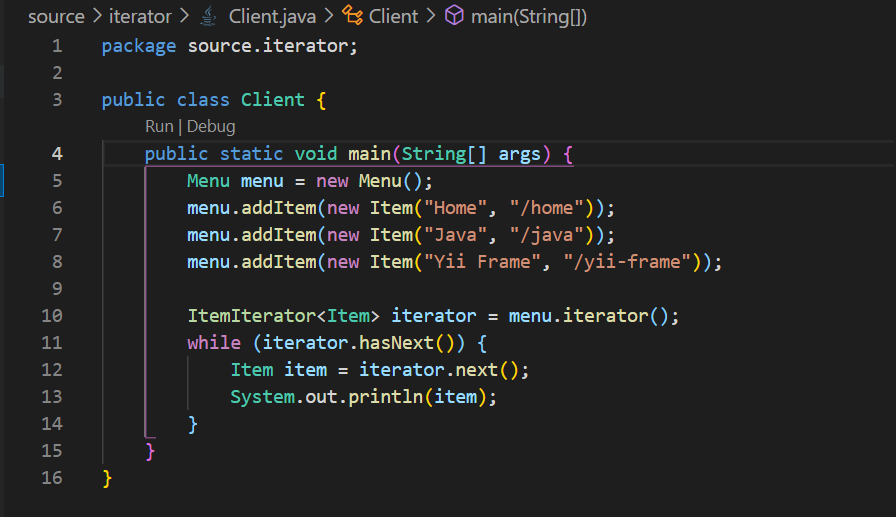
\includegraphics[width=\textwidth]{fig/Iterator/client_class.png}
    \caption{Client Class}
    \label{fig:client_class}
\end{figure}
\begin{figure}
    \centering
    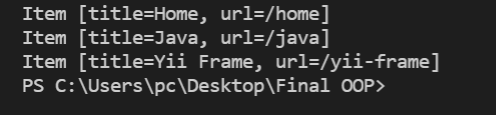
\includegraphics[width=\textwidth]{fig/Iterator/iterator_output.png}
    \caption{Output}
    \label{fig:iterator_output}
\end{figure}

\newpage
\section{Ví dụ thực tế}
\begin{itemize}
    \item Truy xuất nhiều loại tập hợp
    \item Ứng dụng trong chuyển kênh của vô tuyến tuyền hình
    \item Áp dụng trong thư viện java
    \begin{itemize}
        \item java.util.Iterator 
        \item java.util.Enumeration
    \end{itemize}
\end{itemize}


